\section{One-shot Retouching}
\label{sec:Methodology}


\begin{landscape}
\begin{figure*}[th] % "[t!]" placement specifier just for this example
	\centering
	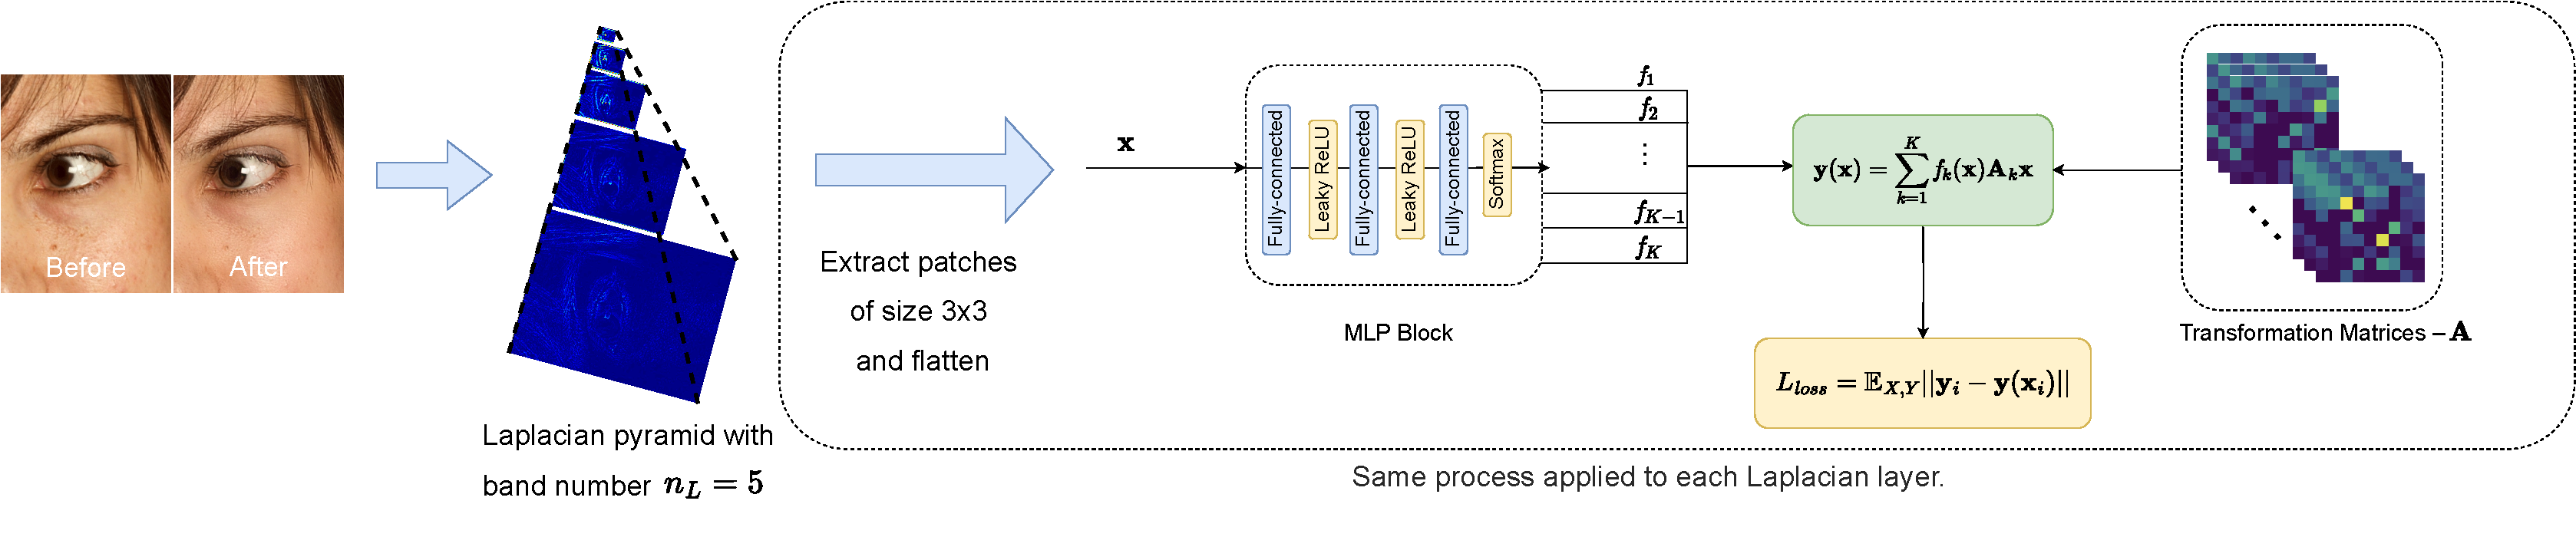
\includegraphics[width=1.5\textwidth]{Chapters/detail-retouching-figs/MainFig.pdf}
    % \includesvg[width=\textwidth]{myfig.svg}
  % \hfill
    \caption{Our technique learns a separate mapping per frequency band by decomposing images into five different bands with a Laplacian pyramid. At each Laplacian band $l$, we define a mapping between flattened patches $\mathbf{x}_i$, $\mathbf{y}_i$ extracted from before-after bands $X_l$, $Y_l$. Our field based method (MLP block) adapts transformations to input patches, providing local context-aware adjustments. The transformation matrices and MLP parameters are learned jointly from scratch for each Laplacian band of the before-after pair.}

\label{fig:modelT}
\end{figure*}
 \end{landscape}


\subsection{Frequency Decomposition}\label{sec:thePatchMap}
% \myworries{Modify equations in the box - transpose is unnecessary}

We first decompose example and input images into different frequency bands by constructing a Laplacian pyramid to capture details at multiple scales. In principle, it is possible to utilize any multiscale image decomposition method. However, we observed that a basic Laplacian pyramid helped us capture more accurate and generalizable results compared to a guided or bilateral pyramid. Therefore, we decompose images by

\begin{equation} 
	X_l = L_l(X) = 
 \left \{ \begin{aligned}
        X - G(2) \ast X \hspace{5mm} &l=0\\
        G(2^l) \ast X - G(2^{l+1}) \ast X \hspace{5mm} &l>0,
       \end{aligned}
 \right.
\end{equation}
where $G(\sigma)$ is the normalized Gaussian kernel, and $\ast$ denotes convolution. We also store the low-pass filtered image $S(X)$ such that $X = S(X) + \sum_{l=0}^{n_L} L_l(X)$. We then downsample each $L_l(X)$ and $S(X)$ according to the maximum frequency present at that band. This allows us to use small $3 \times 3$ patches at each band. In our experiments, we used $n_L = 5$ bands for the Laplacian pyramid.


Since each band is processed independently, we explain the steps of our technique below for two generic images $X$ and $Y$.


\subsection{Transformation Blending}\label{sec:Blending}

The mapping is defined between patches $\mathbf{x} \in \mathbb{R}^{d_X}$ to $\mathbf{y} \in \mathbb{R}^{d_Y}$ extracted from $X$ and $Y$, respectively, where we denote the patches with vectors stacking the pixel values and define the patch spaces as $\mathbb{R}^{d_X}$ and  $\mathbb{R}^{d_Y}$. For all results in this work, we work with $3 \times 3$ patches and thus $d_X = d_Y = 9$.

Our mapping takes the form of a weighted average of learned transformation matrices $\mathbf{A}$, where each transformation matrix $\mathbf{A}_k$ is first multiplied with its corresponding blending weight: 

\begin{equation} 
	\mathbf{y} (\mathbf{x}) = \sum_{k=1}^K
	\mathit{f}_k (\mathbf{x}) \mathbf{A}_k \mathbf{x},
	\label{eq:weightedSum}
\end{equation} 
Here, $K$ is the number of transformation matrices, and $f_k$ are the blending weights, learned by an MLP block of output size $K$. The $\mathbf{A}_k$'s and $f_k$'s are jointly learned by minimizing the following loss on patches extracted from the before and after images.

\begin{equation}
    L_{loss}  = \mathbb{E}_{X, Y} || \mathbf{y}_i -   \mathbf{y} (\mathbf{x}_i) ||
\end{equation}

Each $\mathbf{A}_k$ corresponds to a different type of transformation and the $f_k(\mathbf{x})$'s, represented with the MLP, allow for a smooth transition between different transformations. The form of $f_k$'s is relatively simple with three fully-connected layers and nonlinear activation functions applied after each layer. This blending forms a simple but expressive transformation as we illustrate in the Section \ref{sec:results}.

\subsection{Retouching an Input Image}

We process the input image $I$ the same way as the before-after pair. First, we decompose the input into its Laplacian layers and then extract its patches per layer. After applying the learned mappings $M_l$ to the patches of the corresponding layers $L_{l}(I)$ independently, we then reconstruct the Laplacian bands of the output image $O_l$ by placing the patches at their spatial locations and averaging over the overlapping regions. Later, we obtain the final output image $O$ by summing the outputs $O_l$ and the residual of the input image:
\begin{equation}
    O = S(I) + \sum_{l=0}^{n_L} M_l(L_l(I))\,.
\end{equation}
